\documentclass[11pt]{article}

% =====================================================================
% Packages
% =====================================================================

\usepackage[margin=1in]{geometry}
\usepackage{amsmath, amssymb}
\usepackage{graphicx}
\usepackage{booktabs}
\usepackage{hyperref}
\usepackage{parskip}
\usepackage{xcolor}
\usepackage{listings}

% =====================================================================
% R Code Style
% =====================================================================

\definecolor{codebg}{RGB}{247,247,247}
\definecolor{codecomment}{RGB}{80,130,90}
\definecolor{codekeyword}{RGB}{40,80,150}
\definecolor{codestring}{RGB}{160,70,70}

\lstdefinestyle{rcode}{
    language=R,
    backgroundcolor=\color{codebg},
    basicstyle=\ttfamily\small,
    keywordstyle=\color{codekeyword},
    commentstyle=\color{codecomment}\itshape,
    stringstyle=\color{codestring},
    frame=single,
    rulecolor=\color{black!20},
    breaklines=true,
    showstringspaces=false,
    columns=fullflexible,
    xleftmargin=1.5em,
    xrightmargin=1.5em,
    framexleftmargin=0.8em,
    framexrightmargin=0.8em,
    framesep=0.6em
}

% =====================================================================
% Title
% =====================================================================

\title{MGT 924: Statistical Foundations \\ Problem Set 1}

\author{
    [Your Name] \\
    Group: [Ashley Wen, Emily Wu, Skye Wang, Yiting Huang]
}

\date{\today}

\begin{document}

\maketitle

% =====================================================================
\section{Visualize before building a prediction rule (20 points)}
% =====================================================================

\subsection{Sample Statistics (1.1)}

For each of the four datasets (I, II, III, IV), we computed the following statistics: the mean of \texttt{x}, the mean of \texttt{y},
the variance of \texttt{x}, the variance of \texttt{y}, the correlation
between \texttt{x} and \texttt{y}, and the $R^2$ implied by these
statistics (using the identity $R^2 = r_{xy}^2$ for simple linear
regression).

\begin{table}[h]
\centering
\caption{Sample statistics by dataset}

\begin{tabular}{lcccccc}
\toprule
Dataset & Mean $x$ & Mean $y$ & Var $x$ & Var $y$ & Corr($x,y$) & $R^2$ \\
\midrule
I   & 9 & 7.5009 & 11 & 4.1273 & 0.8164 & 0.6665 \\
II  & 9 & 7.5009 & 11 & 4.1276 & 0.8162 & 0.6662 \\
III & 9 & 7.5000 & 11 & 4.1226 & 0.8163 & 0.6663 \\
IV  & 9 & 7.5009 & 11 & 4.1232 & 0.8165 & 0.6667 \\
\bottomrule
\end{tabular}

\end{table}

% ---------------------------------------------------------------------
\subsection{OLS Estimates (1.2)}
% ---------------------------------------------------------------------

For each dataset, we computedOLS estimates $\hat{\beta}_0$ and $\hat{\beta}_1$ from a regression of \texttt{y} on \texttt{x} using
\texttt{lm()}.

\begin{table}[h]
\centering
\caption{OLS estimates by dataset}

\begin{tabular}{lcc}
\toprule
Dataset & $\hat{\beta}_0$ (Intercept) & $\hat{\beta}_1$ (Slope) \\
\midrule
I   & 3.0001 & 0.5001 \\
II  & 3.0009 & 0.5000 \\
III & 3.0025 & 0.4997 \\
IV  & 3.0017 & 0.4999 \\
\bottomrule
\end{tabular}

\end{table}

% ---------------------------------------------------------------------
\subsection{Trading Rule from Statistics Alone (1.3)}
% ---------------------------------------------------------------------

\textit{Based solely on the statistics computed in 1.1 and 1.2, how
would you trade each of the four stocks?}

\vspace{1em}

\noindent\textbf{Answer:}

From the statistics, we could observe a linear relationship between $x$ and $y$ approximately the same across all four stocks as

\[
\hat{y} = 0.5x + 3,
\]

with a positive correlation of approximately $0.816$ and an $R^2$ of approximately $0.666$. Therefore, I would enter long positions in all four stocks when $x$ is high and short positions when $x$ is low.

% ---------------------------------------------------------------------
\subsection{Scatterplots with OLS Prediction Rule (1.4)}
% ---------------------------------------------------------------------

\begin{figure}[h]
\centering

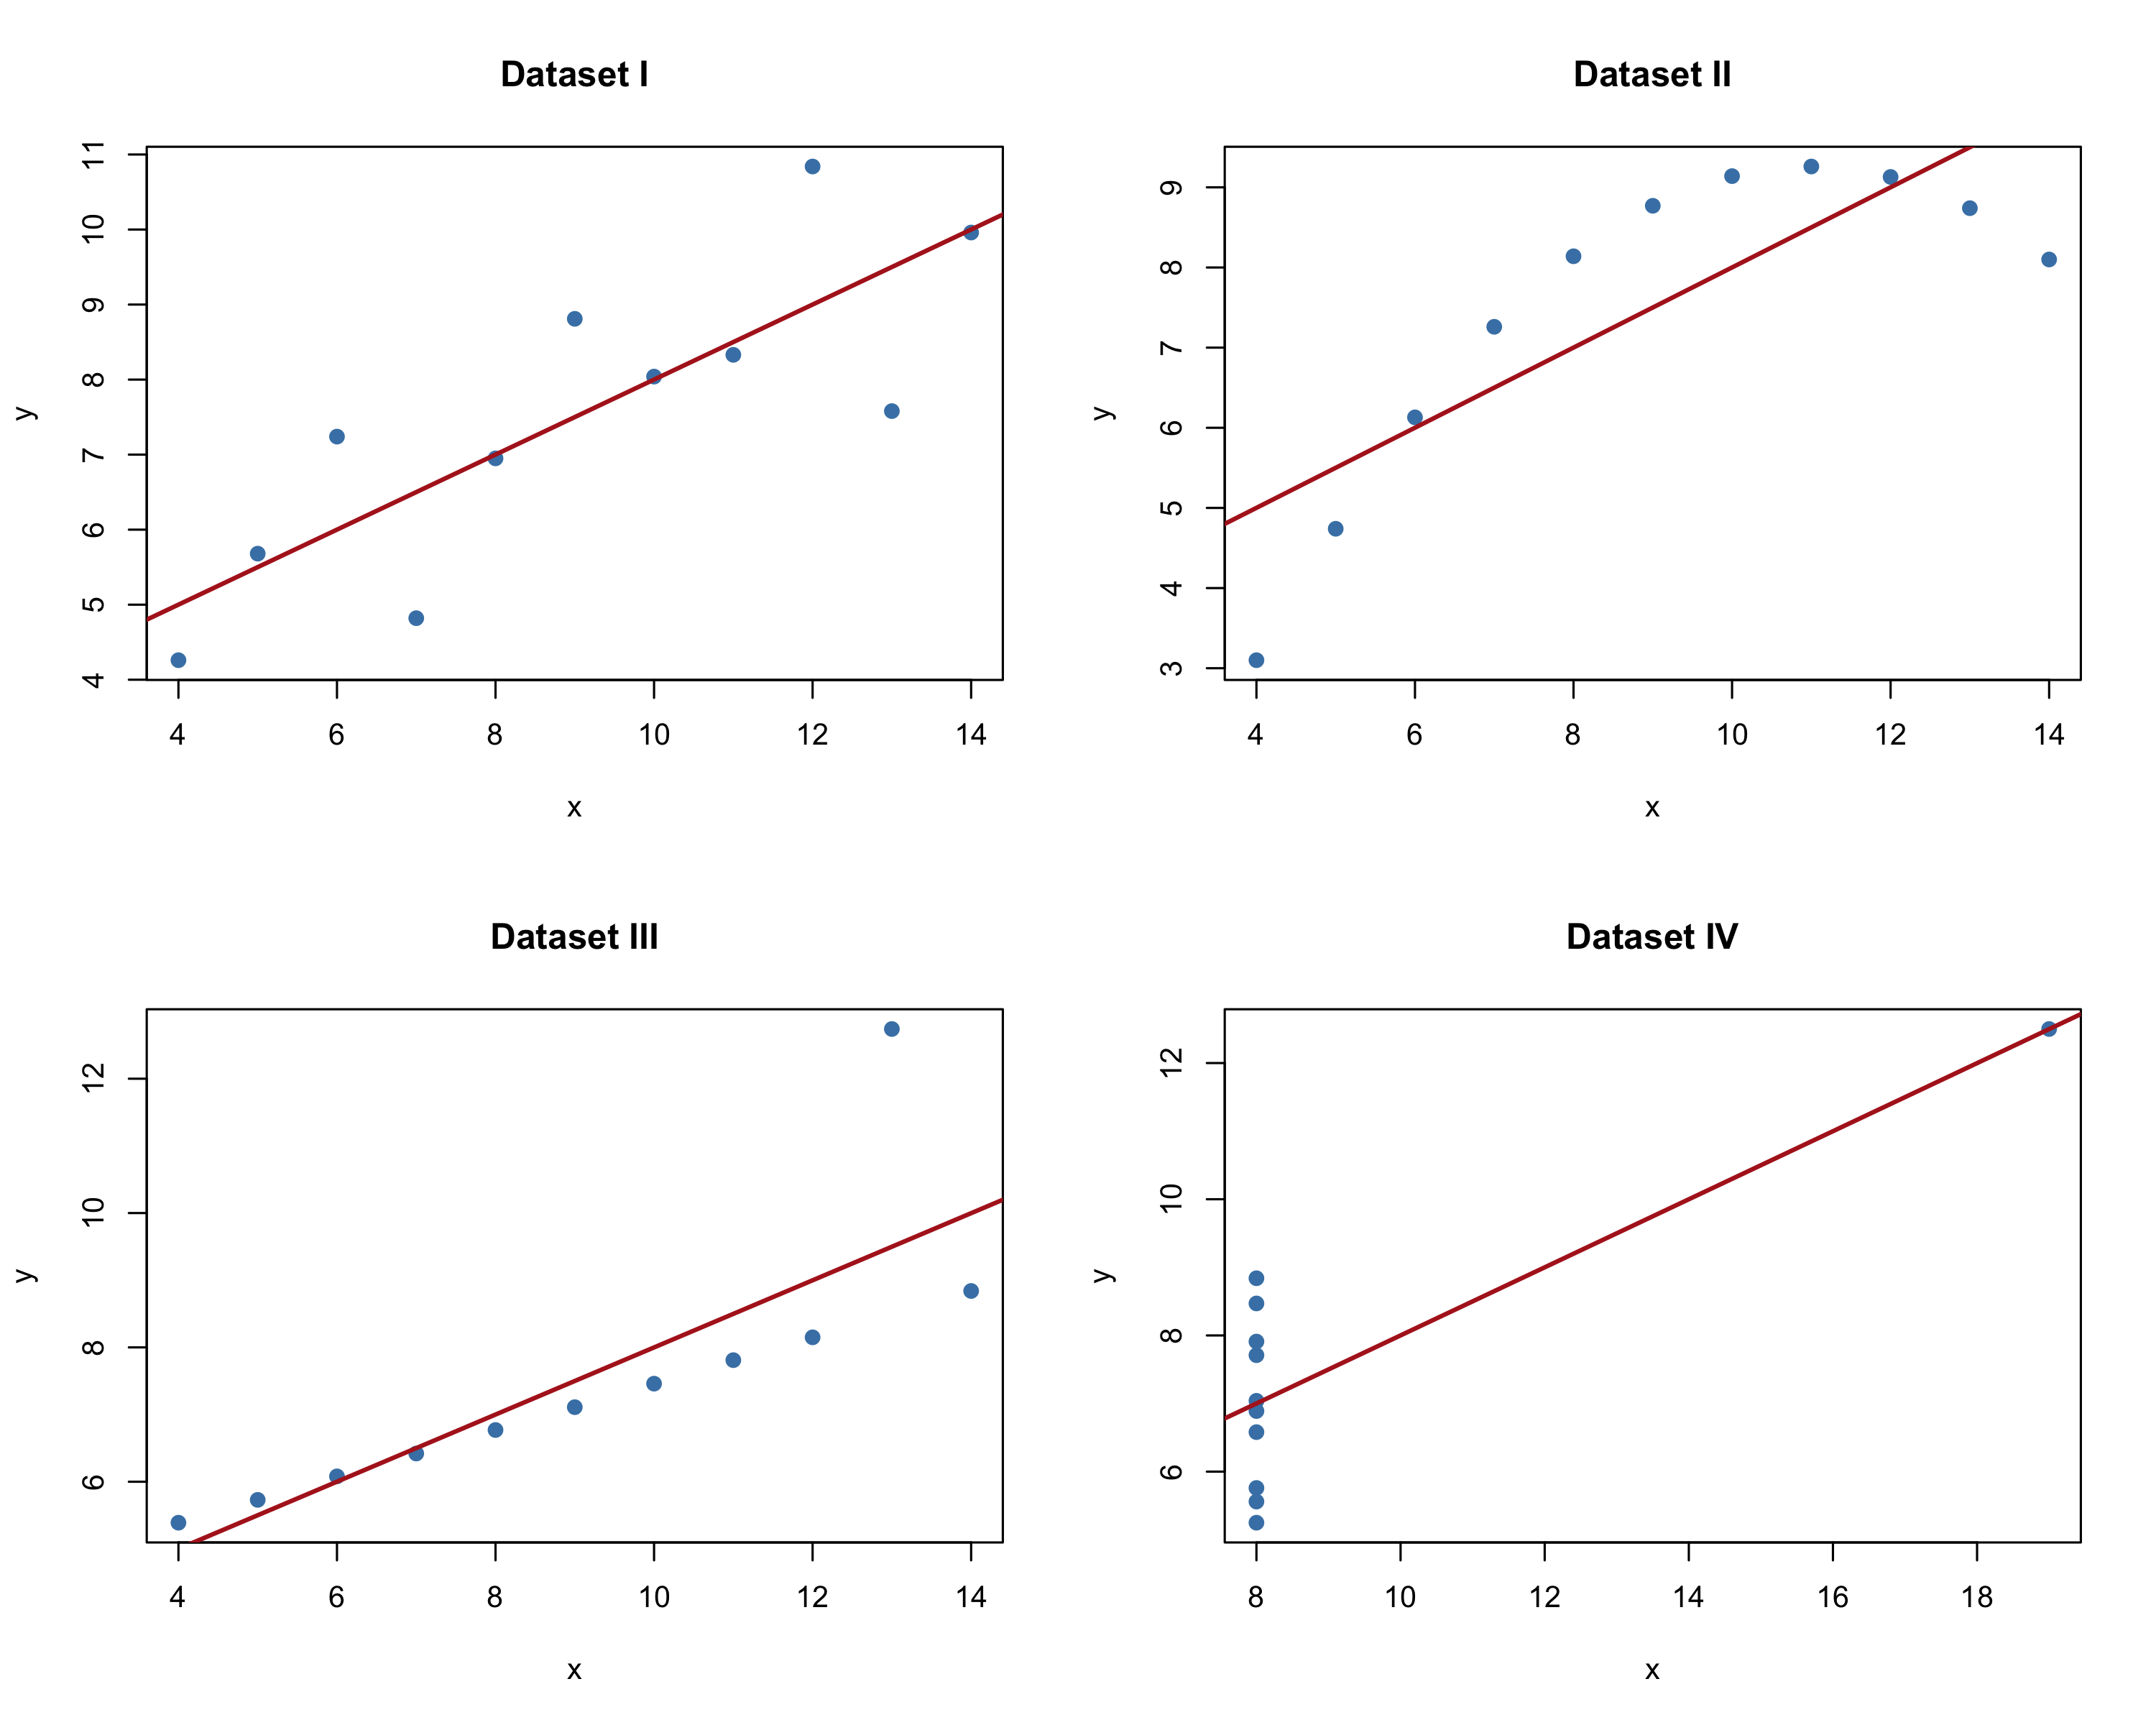
\includegraphics[width=0.85\textwidth]{scatterplots.png}

\caption{Scatterplots of \texttt{y} vs.\ \texttt{x} for each dataset,
with the fitted OLS line overlaid.}

\end{figure}

% ---------------------------------------------------------------------
\subsection{Improving the Trading Strategy (1.5)}
% ---------------------------------------------------------------------

\textit{For each stock, describe the \underline{one} improvement to your
trading strategy (relative to your answer in 1.3) that the scatterplot
suggests is most important.}

\noindent\textbf{Answer:}

Although the four stocks have nearly identical summary statistics and OLS estimates, their scatterplots reveal very different patterns in the relationship between $x$ and $y$. Therefore, the linear trading strategy we proposed in 1.3 should be adjusted separately for each stock based on the structure revealed by the scatterplots.

\vspace{1em}

\noindent\textbf{Dataset I:}

The data points are distributed roughly symmetrically around the fitted line. This suggests the linear relationship provides a reasonable description of the data. Therefore, I would retain the original strategy from 1.3: go long when $x$ is high and short when $x$ is low.

\vspace{1em}

\noindent\textbf{Dataset II:}

The scatterplot shows a clear nonlinear, inverted-U-shaped relationship of $y$ = a$x^2$+b. $y$ initially increases with $x$, but after reaching a peak, the relationship becomes negative. Therefore, I would use different trading rules on the two sides of the turning point: go long as $x$ rises before the peak, but reverse the strategy after the peak and short as $x$ rises further.

\vspace{1em}

\noindent\textbf{Dataset III:}

The scatterplot shows that there is one unusual observation that pulls the entire fitted line upward, making the positive relationship between $x$ and $y$ appear stronger than it is for most of the data. Therefore, I would lower my expectation to the marginal returns. I would still go long when $x$ is high and short when $x$ is low, but with smaller positions and less confidence in the signal.

\vspace{1em}

\noindent\textbf{Dataset IV:}

In this plot, for most observations, there is no clear relationship between $x$ and $y$. The apparent positive linear relationship is driven almost entirely by a single high-leverage observation.

Therefore, I would not rely on the fitted linear rule. And I would avoid taking long or short positions based on $x$ alone without additional evidence.

% =====================================================================
\section{Predicting house prices (40 points)}
% =====================================================================

\subsection{Data Preparation (2.1)}

The following code loads the Connecticut property data, first constructs the
true assessed value, then expresses both assessed value and sale amount in
\$1,000s. Eventually we filters the sample to single-family homes in New Haven
listed in 2008 with true assessed values below \$250,000.

\vspace{0.5em}

\begin{lstlisting}[style=rcode]
# ---- 2.1.1: Load the data ----
ct <- read.csv("ps1/ct_property_data.csv")

# ---- 2.1.2: Create assessedvalue_true ----
# Tax-assessed value in CT is 70% of true market value,
# so dividing by 0.7 recovers the true value.
ct$assessedvalue_true <- ct$assessedvalue / 0.7

# ---- 2.1.3: Express in $1,000s ----
ct$assessedvalue_true <- ct$assessedvalue_true / 1000
ct$saleamount <- ct$saleamount / 1000

# ---- 2.1.4: Filter ----
ct_filtered <- ct[
    ct$residentialtype == "Single Family" &
        ct$town == "New Haven" &
        ct$listyear == 2008 &
        ct$assessedvalue_true < 250,
]
\end{lstlisting}

\vspace{0.5em}

The resulting sample contains \textbf{279 observations}.

% =====================================================================
% Sections 2.2--2.7 are being completed by groupmates.
% Merge their content before final submission.
% =====================================================================

\end{document}